\newpage
\maketitle
\begin{center}
\Large \textbf{第Z01章 深度学习框架} \quad 
\end{center}
\begin{abstract}
在本章中我们将利用Numpy开发一个小型的深度学习框架,实现类似PyTorch的功能。
\end{abstract}
\section{深度学习框架概述}
在本章中,我们将利用Numpy,开发一个基于动态计算图的深度学习框架。
\subsection{张量}
在深度学习中,最基本的元素是张量(Tensor)。1维张量就是我们所熟悉的向量,2维张量就是矩阵,3维及以上就是通用的张量。张量(Tensor)在
Numpy中就用多维数组来表示。
我们首先定义一个仅支持加法运算,但是支持自动微分的张量原型,在后面的章节在逐渐扩充完善。
\subsubsection{最简张量模型}
我们首先定义一个最简单的张量,如下所示:
\lstset{language=PYTHON, caption={策略迭代(chpZ01/tensor.py)}, label={chpZ01-simple-tensor}}
\begin{lstlisting}
import numpy as np

class Tensor(object):
	def __init__(self, data, autograd=False, creators=None, creation_op=None, cid=None):
		self.data =np.array(data)
		self.creators = creators
		self.creation_op = creation_op
		self.autograd = autograd
		self.grad = None
		self.children = {}
		if (cid is None):
			cid = np.random.randint(0, 10000000)
		self.cid = cid
		if creators is not None:
			for c in creators:
				if self.cid not in c.children:
					c.children[self.cid] = 1
				else:
					c.children[self.cid] += 1

	def all_children_grads_accounted_for(self):
		for cid, cnt in self.children.items():
			if cnt != 0:
				return False
		return True

	def backward(self, grad=None, grad_origin=None):
		if self.autograd:
			if grad_origin is not None:
				if self.children[grad_origin.cid] == 0:
					raise Exception('cannot backprop more than once')
				else:
					self.children[grad_origin.cid] -= 1
			if self.grad is None:
				self.grad = grad
			else:
				self.grad += grad
			if self.creators is not None and (self.all_children_grads_accounted_for() or grad_origin is None):
				if self.creation_op == 'add':
					self.creators[0].backward(self.grad, self)
					self.creators[1].backward(self.grad, self)

	def __add__(self, other):
		if self.autograd and other.autograd:
			return Tensor(self.data + other.data, autograd=True, creators=[self, other], creation_op='add')
		return Tensor(self.data + other.data)

	def __repr__(self):
		return str(self.data.__repr__())

	def __str__(self):
		return str(self.data.__str__())

	def to_string(self):
		ts = 'tensor_{0}:\r\n'.format(self.cid)
		ts = '{0}    data:{1};\r\n'.format(ts, self.data)
		ts = '{0}    autograd: {1};\r\n'.format(ts, self.autograd)
		ts = '{0}    creators: {1};\r\n'.format(ts, self.creators)
		ts = '{0}    creation_op: {1};\r\n'.format(ts, self.creation_op)
		ts = '{0}    cid: {1};\r\n'.format(ts, self.cid)
		ts = '{0}    grad: {1};\r\n'.format(ts, self.grad)
		ts = '{0}    children: {1};\r\n'.format(ts, self.children)
		return ts
\end{lstlisting}
直接看代码比较难以理解,下面我们先写一个单元测试用例,实现一个前向传播过程,如下所示:
\lstset{language=PYTHON, caption={向量前向传播测试用例(chpZ01/tensor.py)}, label={chpZ01-simple-tensor-forward-unit-test001}}
\begin{lstlisting}
class TTensor(unittest.TestCase):
    @classmethod
    def setUp(cls):
        pass

    @classmethod
    def tearDown(cls):
        pass

    def test_init_001(self):
        a = Tensor([1, 2, 3, 4, 5], autograd=True)
        b = Tensor([10, 10, 10, 10, 10], autograd=True)
        c = Tensor([5, 4, 3, 2, 1], autograd=True)
        d = a + b
        e = b + c
        f = d + e
        print('f: {0};'.format(f.to_string()))
        print('d: {0};'.format(d.to_string()))
        print('e: {0};'.format(e.to_string()))
        print('a: {0};'.format(a.to_string()))
        print('b: {0};'.format(b.to_string()))
        print('c: {0};'.format(c.to_string()))
\end{lstlisting}
运行上面的测试用例:
\lstset{language=BASH, caption={向量前向传播测试用例运行(chpZ01/tensor.py)}, label={chpZ01-simple-tensor-forward-unit-test001-run}}
\begin{lstlisting}
python -m unittest uts.apps.drl.chpZ01.t_tensor.TTensor.test_init_001
\end{lstlisting}
运行结果如下所示:
\begin{figure}[h]
	\caption{向量前向传播执行结果}
	\label{p000015}
	\centering
	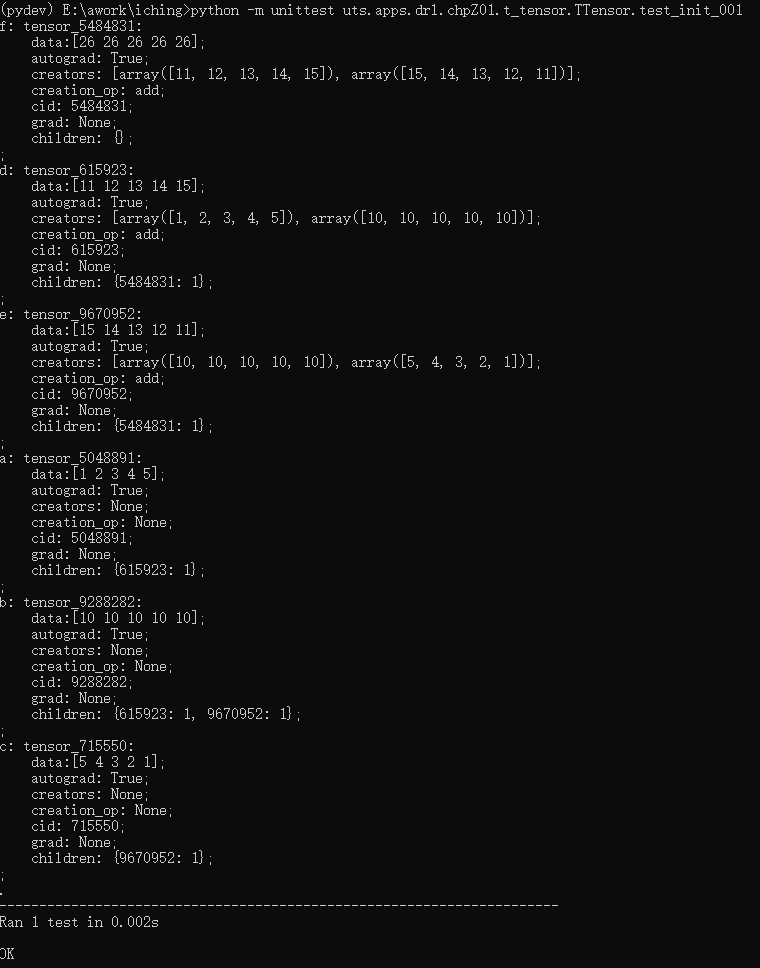
\includegraphics[height=10cm]{images/p000015}
\end{figure}
其将形成如下所示的动态图:
\begin{figure}[h]
	\caption{向量加法动态图示例}
	\label{p000016}
	\centering
	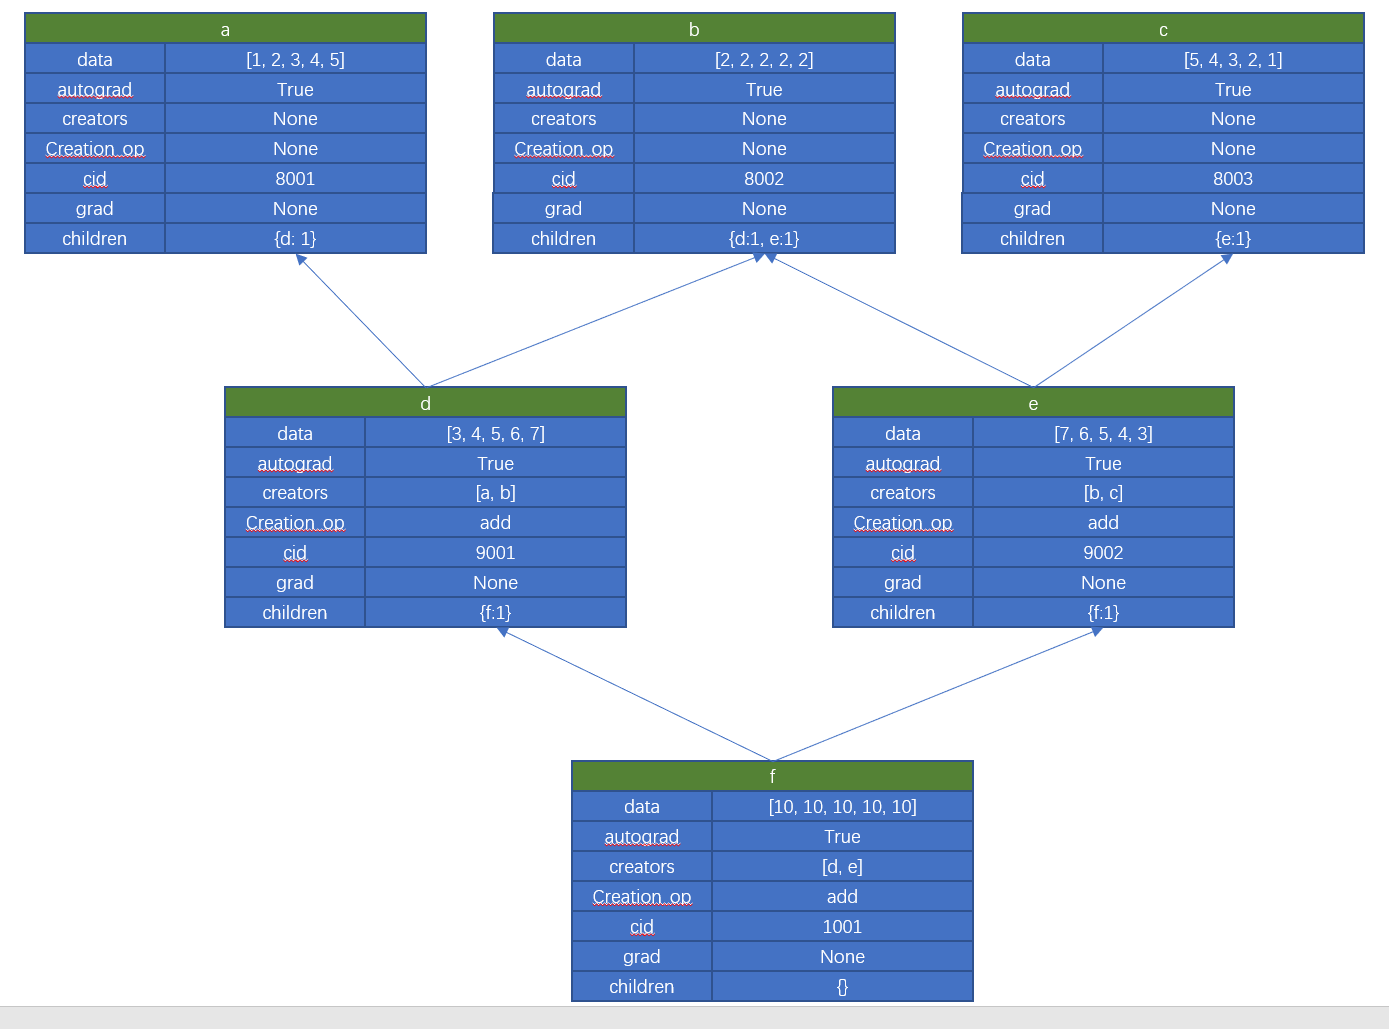
\includegraphics[height=10cm]{images/p000016}
\end{figure}
接下来我们看一下反向传播过程,首先来看测试用例:
\lstset{language=PYTHON, caption={向量前向传播测试用例(chpZ01/tensor.py)}, label={chpZ01-simple-tensor-forward-unit-test001}}
\begin{lstlisting}
class TTensor(unittest.TestCase):

	def test_add_backward_001(self):
		a = Tensor([1, 2, 3, 4, 5], autograd=True)
		b = Tensor([10, 10, 10, 10, 10], autograd=True)
		c = Tensor([5, 4, 3, 2, 1], autograd=True)
		d = a + b
		e = b + c
		f = d + e
		f.backward(Tensor([1, 1, 1, 1, 1]))
		print('f: {0};'.format(f.to_string()))
		print('d: {0};'.format(d.to_string()))
		print('e: {0};'.format(e.to_string()))
		print('a: {0};'.format(a.to_string()))
		print('b: {0};'.format(b.to_string()))
		print('c: {0};'.format(c.to_string()))
\end{lstlisting}
我们首先来看理论分析,对于$f=d+e $,我们先定$\frac{\partial j}{\partial f}=[1, 1, 1, 1, 1]$,根据链式求导法则,得到$\frac{\partial j}{\partial \boldsymbol{e}}=\frac{\partial j}{\partial \boldsymbol{f}} \frac{\partial \boldsymbol{f}}{\partial \boldsymbol{e}}$,
向量对向量微分是得到的是Jacobian矩阵,如下所示:
\begin{equation}
\begin{aligned}
\frac{\partial \boldsymbol{f}}{\partial \boldsymbol{e}} = \begin{bmatrix}
\frac{\partial f_{1}}{\partial e_{1}} & \frac{\partial f_{1}}{\partial e_{2}} & ... & \frac{\partial f_{1}}{\partial e_{n}} \\
\frac{\partial f_{2}}{\partial e_{1}} & \frac{\partial f_{2}}{\partial e_{2}} & ... & \frac{\partial f_{2}}{\partial e_{n}} \\
... & ... & ... & ... \\
\frac{\partial f_{n}}{\partial e_{1}} & \frac{\partial f_{n}}{\partial e_{2}} & ... & \frac{\partial f_{n}}{\partial e_{n}}
\end{bmatrix} \in R^{n \times n}
\end{aligned}
\label{chpZ01-vector-vector-gradient}
\end{equation}
其实际执行为$R^{1 \times n} \cdot R^{n \times n}=R^{1 \times n}$,以上为理论分析,下面我来看程序上面的代码实现。
对于向量$\boldsymbol{f}$,我们直接指定$\frac{\partial j}{\partial \boldsymbol{f}}=[1, 1, 1, 1, 1]$,向量$\boldsymbol{f}$当前状态为:
\begin{figure}[h]
	\caption{向量f原始状态}
	\label{p000017}
	\centering
	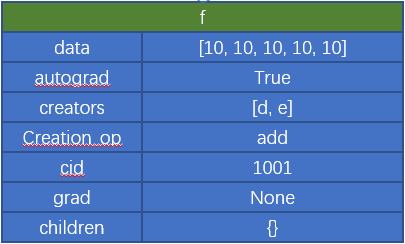
\includegraphics[height=5cm]{images/p000017}
\end{figure}
反向传播程序如下所示:
\lstset{language=PYTHON, caption={向量前向传播测试用例(chpZ01/tensor.py)}, label={chpZ01-simple-tensor-backward-f}}
\begin{lstlisting}
    def backward(self, grad=None, grad_origin=None):
        if self.autograd:
            if grad_origin is not None:
                if self.children[grad_origin.cid] == 0:
                    raise Exception('cannot backprop more than once')
                else:
                    self.children[grad_origin.cid] -= 1
            if self.grad is None:
                self.grad = grad
            else:
                self.grad += grad
            if self.creators is not None and (self.all_children_grads_accounted_for() or grad_origin is None):
                if self.creation_op == 'add':
                    self.creators[0].backward(self.grad, self)
                    self.creators[1].backward(self.grad, self)
\end{lstlisting}
代码解读如下所示:
\begin{itemize}
	\item 第2行:因为autograd为True,所以执行下面的代码;
	\item 第3$\sim$7行:因为grad\_origin为False,所以不执行;
	\item 第8$\sim$11行:因为grad为None,因此执行第9行使$grad=[1, 1, 1, 1, 1]$;
	\item 第12行:因为creators为d和e,且all\_children\_grads\_accounted\_for为True,且grad\_origin为None,因此会执行下面的语句;
	\item 第13$\sim$15行:由于是add运算,以自己的grad和自身为参数,分别调用d和e的后向传播算法;
\end{itemize}
执行完上述代码后,系统状态如下所示:
\begin{figure}[h]
	\caption{反向传播从f到d和e}
	\label{p000018}
	\centering
	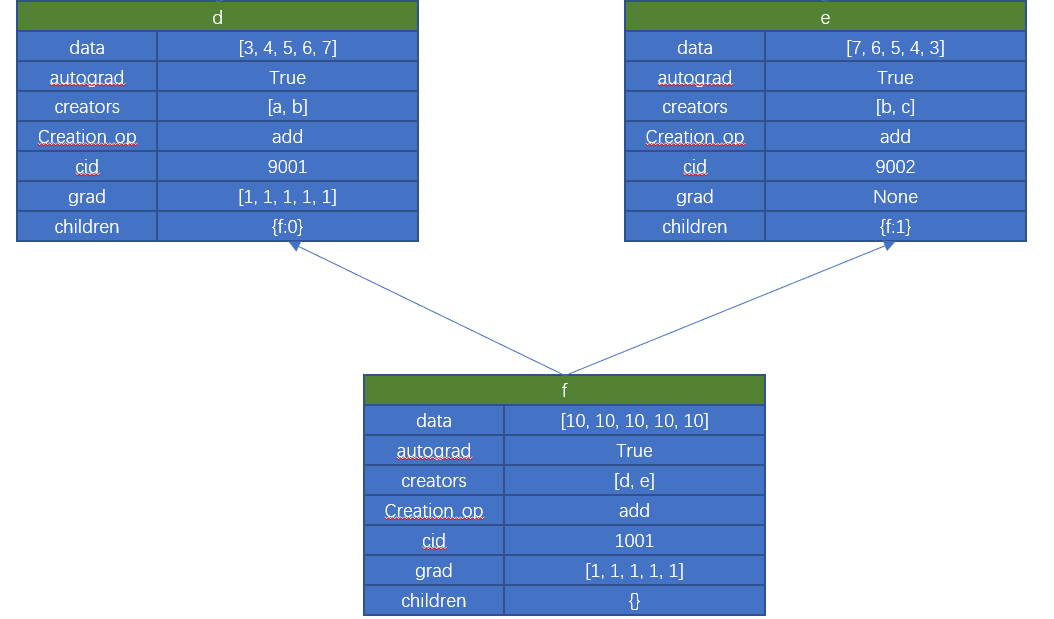
\includegraphics[width=10cm]{images/p000018}
\end{figure}
我们先来看传到d节点,这时grad\_origin为f,此时d的children只有一个节点f,初始时children[f.cid]=1,运行后children[f.cid]=0,因为self.grad为空,
所以self.grad=[1, 1, 1, 1, 1],因为self.creators=[a, b],又为add操作,所以会调用a和b的反向传播算法。
\begin{figure}[h]
	\caption{反向传播从d到a和b}
	\label{p000019}
	\centering
	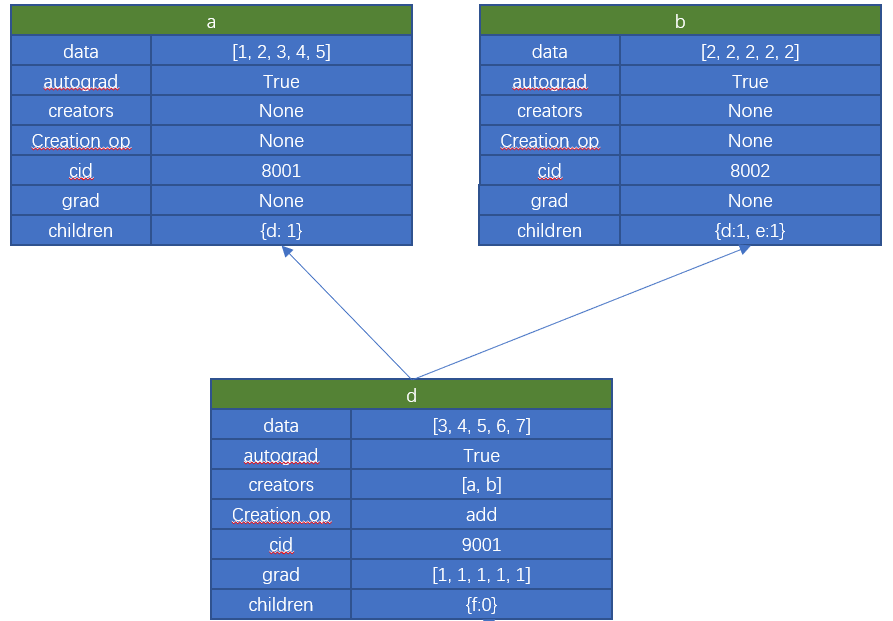
\includegraphics[width=10cm]{images/p000019}
\end{figure}
经过a和b的反向传播算法处理后,结果如下所示:
\begin{figure}[h]
	\caption{反向传播从d到a和b后的处理结果}
	\label{p000020}
	\centering
	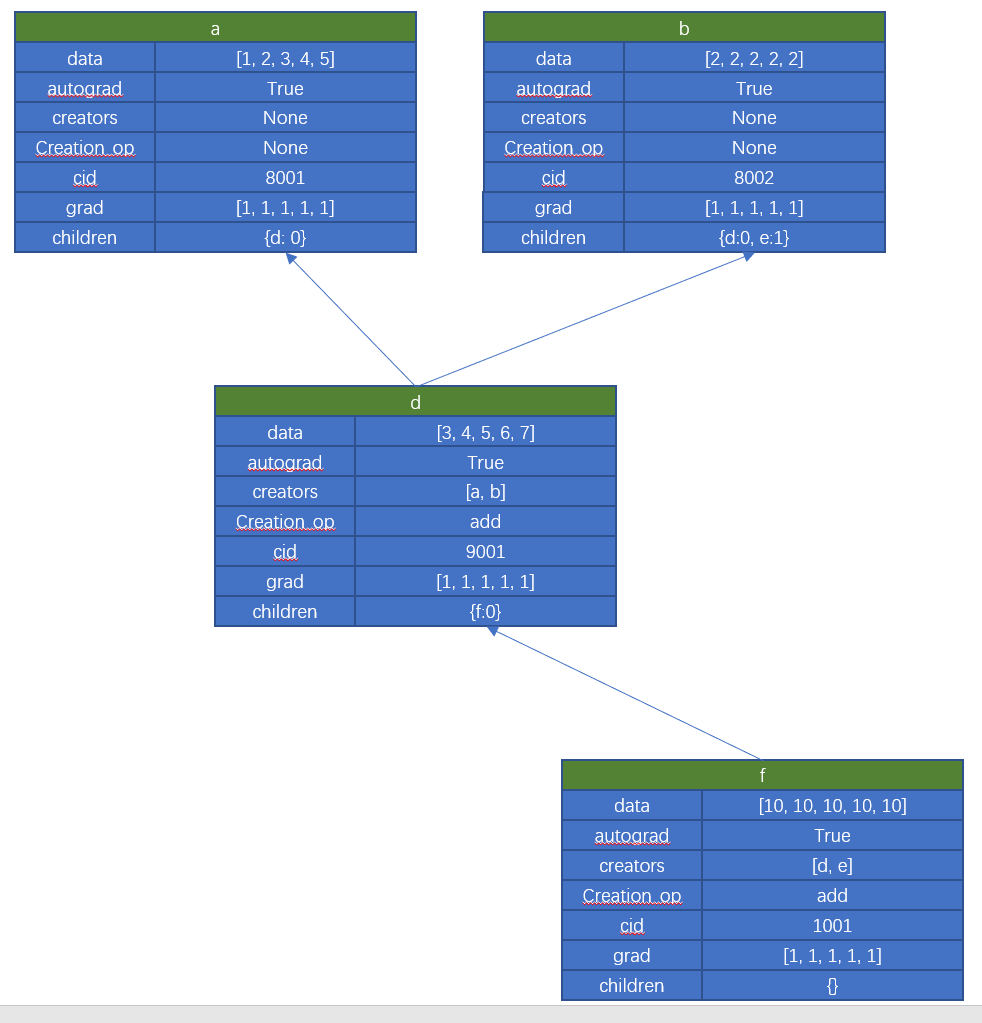
\includegraphics[width=10cm]{images/p000020}
\end{figure}
我们再来看传到e节点,这时grad\_origin为f,此时d的children只有一个节点f,初始时children[f.cid]=1,运行后children[f.cid]=0,因为self.grad为空,
所以self.grad=[1, 1, 1, 1, 1],因为self.creators=[a, b],又为add操作,所以会调用b和c的反向传播算法。
\begin{figure}[h]
	\caption{反向传播从e到b和c}
	\label{p000021}
	\centering
	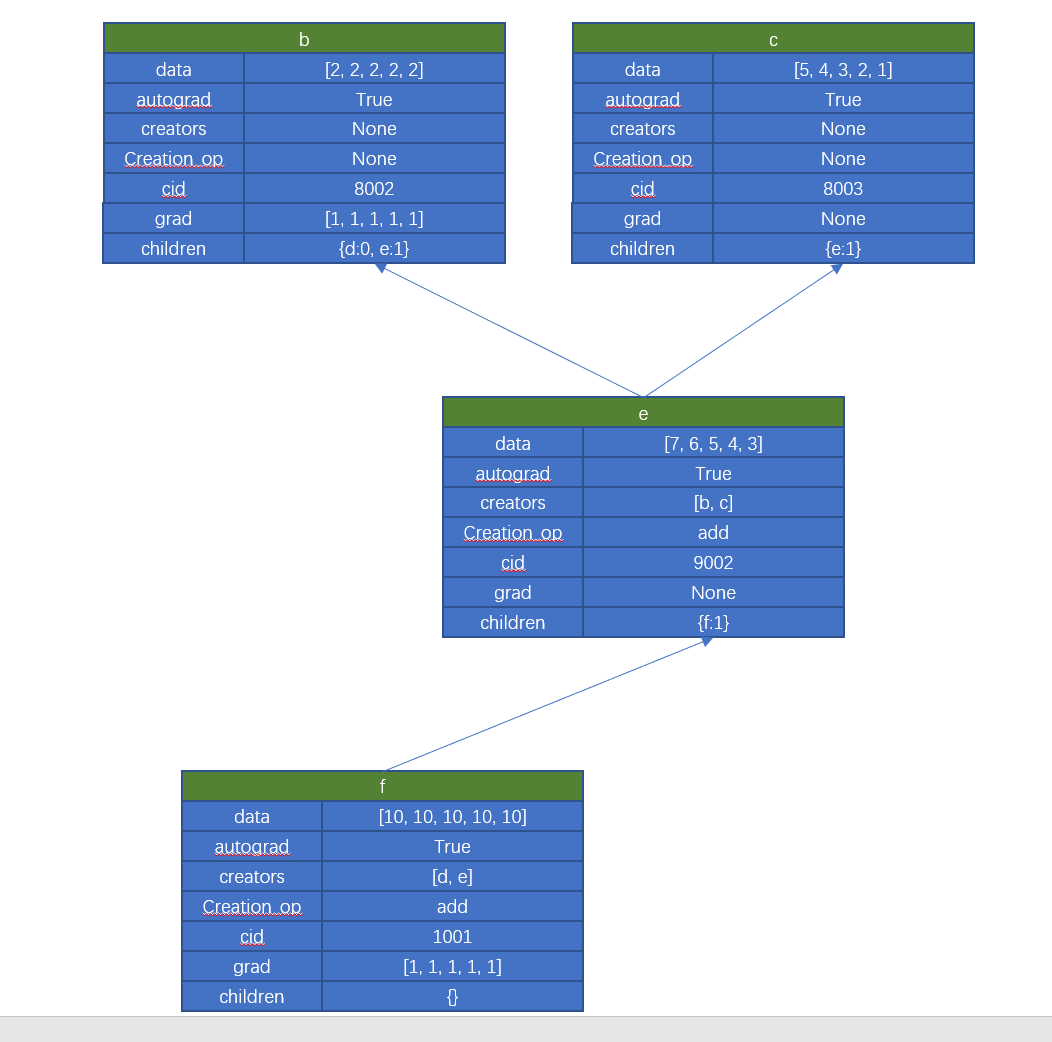
\includegraphics[width=10cm]{images/p000021}
\end{figure}
经过b和c的反向传播算法处理后,结果如下所示:
\begin{figure}[h]
	\caption{反向传播从e到b和c后的处理结果}
	\label{p000022}
	\centering
	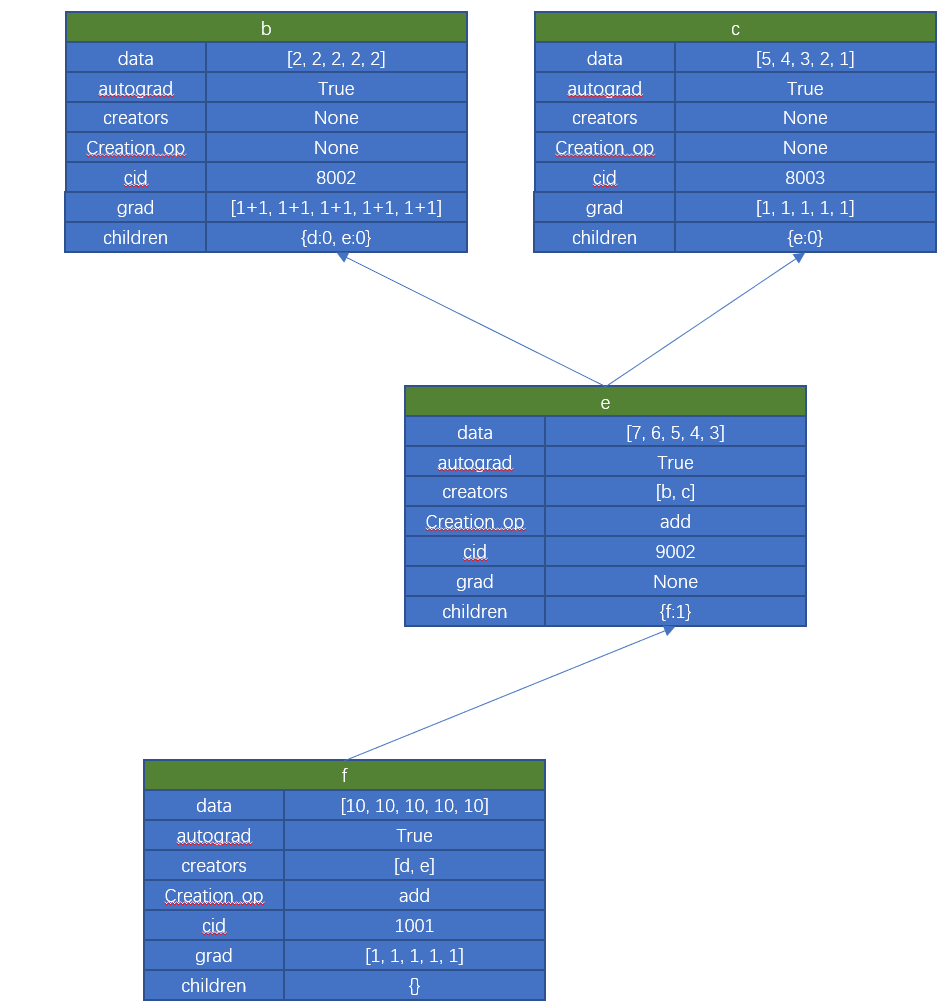
\includegraphics[width=10cm]{images/p000022}
\end{figure}

\subsubsection{负号}
我们首先定义负号方法:
\lstset{language=PYTHON, caption={张量负号方法(chpZ01/tensor.py)}, label={chpZ01-tensor-neg-def}}
\begin{lstlisting}
    def __neg__(self):
        if self.autograd:
            return Tensor(self.data * -1, autograd=True, creators=[self], creation_op='neg')
        return Tensor(self.data * -1)
\end{lstlisting}
其后向传播定义为:
\lstset{language=PYTHON, caption={张量负号反向传播(chpZ01/tensor.py)}, label={chpZ01-tensor-neg-backward}}
\begin{lstlisting}
    def backward(self, grad=None, grad_origin=None):
        if self.autograd:
            if grad_origin is not None:
                if self.children[grad_origin.cid] == 0:
                    raise Exception('cannot backprop more than once')
                else:
                    self.children[grad_origin.cid] -= 1
            if self.grad is None:
                self.grad = grad
            else:
                self.grad += grad
            if self.creators is not None and (self.all_children_grads_accounted_for() or grad_origin is None):
                if self.creation_op == 'add':
                    self.creators[0].backward(self.grad, self)
                    self.creators[1].backward(self.grad, self)
                elif self.creation_op == 'neg':
                    self.creators[0].backward(self.grad.__neg__())
\end{lstlisting}

\subsubsection{减法}
我们首先定义减法:
\lstset{language=PYTHON, caption={张量减法(chpZ01/tensor.py)}, label={chpZ01-tensor-sub-def}}
\begin{lstlisting}
    def __sub__(self, other):
        if self.autograd:
            return Tensor(self.data - other.data, autograd=True, creators=[self, other], creation_op='sub')
        return Tensor(self.data - other.data)
\end{lstlisting}
减法的后向传播定义为:
\lstset{language=PYTHON, caption={张量减法后台传播(chpZ01/tensor.py)}, label={chpZ01-tensor-sub-backward}}
\begin{lstlisting}
    def backward(self, grad=None, grad_origin=None):
        if self.autograd:
            if grad_origin is not None:
                if self.children[grad_origin.cid] == 0:
                    raise Exception('cannot backprop more than once')
                else:
                    self.children[grad_origin.cid] -= 1
            if self.grad is None:
                self.grad = grad
            else:
                self.grad += grad
            if self.creators is not None and (self.all_children_grads_accounted_for() or grad_origin is None):
                if self.creation_op == 'add':
                    self.creators[0].backward(self.grad, self)
					self.creators[1].backward(self.grad, self)
				......
                elif self.creation_op == 'sub':
                    org = Tensor(self.grad.data)
                    self.creators[0].backward(org, self)
                    org = Tensor(self.grad.__neg__().data)
                    self.creators[1].backward(org, self)
\end{lstlisting}


\subsubsection{乘法}
我们首先定义乘法,这里的乘法是指对*运算符的重载,就是两个数组对应元素相乘(Elementwise Multiplication),不是我们将在后面介绍的
矩阵和向量的乘法:
\lstset{language=PYTHON, caption={张量乘法(chpZ01/tensor.py)}, label={chpZ01-tensor-mul-def}}
\begin{lstlisting}
    def __mul__(self, other):
        if self.autograd and other.autograd:
            return Tensor(self.data * other.data, autograd=True, creators=[self, other], creation_op='mul')
        return Tensor(self.data * other.data)
\end{lstlisting}
乘法反向传播算法:
\lstset{language=PYTHON, caption={张量乘法反向传播(chpZ01/tensor.py)}, label={chpZ01-tensor-mul-backward}}
\begin{lstlisting}
    def backward(self, grad=None, grad_origin=None):
        if self.autograd:
            if grad_origin is not None:
                if self.children[grad_origin.cid] == 0:
                    raise Exception('cannot backprop more than once')
                else:
                    self.children[grad_origin.cid] -= 1
            if self.grad is None:
                self.grad = grad
            else:
                self.grad += grad
            if self.creators is not None and (self.all_children_grads_accounted_for() or grad_origin is None):
                if self.creation_op == 'add':
                    self.creators[0].backward(self.grad, self)
					self.creators[1].backward(self.grad, self)
				......
                elif self.creation_op == 'mul':
                    rst = self.grad * self.creators[1]
                    self.creators[0].backward(rst, self)
                    rst = self.grad * self.creators[0]
                    self.creators[1].backward(rst, self)
\end{lstlisting}
从数学概念上来看,两个向量Elementwise相乘之后,得到的是同维度的向量,再求出的微分是一个矩阵,如下所示:
\begin{equation}
\begin{aligned}
\boldsymbol{c} = \boldsymbol{a} * \boldsymbol{b} = \begin{bmatrix}
	c_{1} & c{2} & ... & c_{n}
\end{bmatrix} = \begin{bmatrix}
	a_{1}*b_{1} & a_{2}*b_{2} & ... & a{n}*b{n}
\end{bmatrix} \in R^{n}
\end{aligned}
\label{chpZ01-vector-elementwise-mul}
\end{equation}
我们要求的$\frac{\partial \boldsymbol{c}}{\partial \boldsymbol{a}}$是一个向量对向量的微分,其为一个$R^{n \times n}$的矩阵,如下所示:
\begin{equation}
\begin{aligned}
\frac{\partial \boldsymbol{c}}{\partial \boldsymbol{a}} = \begin{bmatrix}
	\frac{\partial c_{1}}{\partial a_{1}} & \frac{\partial c_{1}}{\partial a_{2}} & ... & \frac{\partial c_{1}}{\partial a_{n}} \\
	\frac{\partial c_{2}}{\partial a_{1}} & \frac{\partial c_{2}}{\partial a_{2}} & ... & \frac{\partial c_{2}}{\partial a_{n}} \\
	... & ... & ... & ... \\
	\frac{\partial c_{n}}{\partial a_{1}} & \frac{\partial c_{n}}{\partial a_{2}} & ... & \frac{\partial c_{n}}{\partial a_{n}}
\end{bmatrix}  = \begin{bmatrix}
	b_{1} & 0 & ... & 0 \\
	0 & b_{2} & ... & 0 \\
	... & ... & ... & ... \\
	0 & 0 & ... & b_{n}
\end{bmatrix} \in R^{n \times n}
\end{aligned}
\label{chpZ01-vector-elementwise-mul}
\end{equation}
我们上面的结果就是这个矩阵对角线的值。

\subsubsection{sum运算}
我们首先来看sum运算,其有一个参数dim,表明要对哪维操作(即消除哪维),例如v.sum(0),就是消除行,如下所示:
\begin{equation}
\begin{aligned}
sum(v, 0)=sum(\begin{bmatrix}
	1 & 2 & 3 & 4 & 5 \\
	2 & 3 & 4 & 5 & 6 \\
	6 & 7 & 9 & 10 & 11 
\end{bmatrix}, 0)=\begin{bmatrix}
	9 & 12 & 16 & 19 & 22
\end{bmatrix}
\end{aligned}
\label{chpZ01-sum-dim-0-demo}
\end{equation}
同理sum(1)如下所示:
\begin{equation}
\begin{aligned}
sum(v, 0)=sum(\begin{bmatrix}
	1 & 2 & 3 & 4 & 5 \\
	2 & 3 & 4 & 5 & 6 \\
	6 & 7 & 8 & 9 & 10 
\end{bmatrix}, 0)=\begin{bmatrix}
	15 \\
	20 \\
	40
\end{bmatrix}
\end{aligned}
\label{chpZ01-sum-dim-1-demo}
\end{equation}
接下来我们来看expand操作,其有两个操作,第1个参数是扩展哪维,第2个参数是重复几份,如下所示:
\lstset{language=PYTHON, caption={张量expand示例(chpZ01/tensor.py)}, label={chpZ01-tensor-expand-demo-1}}
\begin{lstlisting}
org: [
	[1, 2, 3],
	[4, 5, 6]
]
expand(0, 4):
[
	[
		[1, 2, 3],
		[4, 5, 6]
	],
	[
		[1, 2, 3],
		[4, 5, 6]
	],
	[
		[1, 2, 3],
		[4, 5, 6]
	],
	[
		[1, 2, 3],
		[4, 5, 6]
	]
]
expand(1, 4):
[
	[
		[1, 1, 1, 1],
		[2, 2, 2, 2],
		[3, 3, 3, 3]
	],
	[
		[4, 4, 4, 4],
		[5, 5, 5, 5],
		[6, 6, 6, 6]
	]
]
\end{lstlisting}
下面我们来看具体的代码实现:
\lstset{language=PYTHON, caption={张量expand示例(chpZ01/tensor.py)}, label={chpZ01-tensor-sum-expand-code}}
\begin{lstlisting}
    def sum(self, dim):
        if self.autograd:
            return Tensor(self.data.sum(dim), autograd=True, creators=[self], creation_op='sum_' + str(dim))
        return Tensor(self.data.sum(dim))

    def expand(self, dim, copies):
        trans_cmd = list(range(0, len(self.data.shape)))
        trans_cmd.insert(dim, len(self.data.shape))
        new_shape = list(self.data.shape) + [copies]
        new_data = self.data.repeat(copies).reshape(new_shape)
        new_data = new_data.transpose(trans_cmd)
        if self.autograd:
            return Tensor(new_data, autograd=True, creators=[self], creation_op='expand_'+str(dim))
        return Tensor(new_data)
\end{lstlisting}
代码解读如下所示:
\begin{itemize}
	\item 第1$\sim$4行:定义sum运算,其直接调用numpy的sum函数,比较简单;
	\item 第6行:定义expand运算,我们以上例中$v=[[1, 2, 3],[4, 5, 6]] \in R^{2 \times 3}$为例进行讲解,我们先来看$dim=0, copies=4$的情况;
	\item 第7行:$trans_cmd$为$[0, 1]$;
	\item 第8行:$trans_cmd$为$[2, 0, 1]$,因为$len(self.data.shape)$的值为2,当$dim=0$时,在列表最前面插入;
	\item 第9行:$new_shape$为$[2, 3, 4]$;
	\item 第10行:$self.data.repeat(4)$后为$R^{24}$的数组$[1 1 1 1 2 2 2 2 3 3 3 3 4 4 4 4 5 5 5 5 6 6 6 6]$,将其重新定义为$R^{2 \times 3 \times 4}$,其值如下所
	示:
	\lstset{language=PYTHON, caption={张量expand代码解读1(chpZ01/tensor.py)}, label={chpZ01-tensor-expand-code-1}}
	\begin{lstlisting}
	[
		[
			[1 1 1 1]
			[2 2 2 2]
			[3 3 3 3]
		]
		[
			[4 4 4 4]
			[5 5 5 5]
			[6 6 6 6]
		]
	]
	\end{lstlisting}
	\item 第11行:将最后1维放到前面,如下所示:
	\lstset{language=PYTHON, caption={张量expand代码解读1(chpZ01/tensor.py)}, label={chpZ01-tensor-expand-code-2}}
	\begin{lstlisting}
	[
		[
			[1 2 3]
			[4 5 6]
		]
		[
			[1 2 3]
			[4 5 6]
		]
		[
			[1 2 3]
			[4 5 6]
		]
		[
			[1 2 3]
			[4 5 6]
		]
	]
	\end{lstlisting}	
	\item 第6行:定义expand运算,我们以上例中$v=[[1, 2, 3],[4, 5, 6]] \in R^{2 \times 3}$为例进行讲解,我们先来看$dim=1, copies=4$的情况;
	\item 第7行:$trans_cmd$为$[0, 1]$;
	\item 第8行:$trans_cmd$为$[0, 2, 1]$,因为$len(self.data.shape)$的值为2,当$dim=0$时,在列表最前面插入;
	\item 第9行:$new_shape$为$[2, 3, 4]$;
	\item 第10行:$self.data.repeat(4)$后为$R^{24}$的数组$[1 1 1 1 2 2 2 2 3 3 3 3 4 4 4 4 5 5 5 5 6 6 6 6]$,将其重新定义为$R^{2 \times 3 \times 4}$,其值如下所
	示:
	\lstset{language=PYTHON, caption={张量expand代码解读1(chpZ01/tensor.py)}, label={chpZ01-tensor-expand-code-3}}
	\begin{lstlisting}
	[
		[
			[1 1 1 1]
			[2 2 2 2]
			[3 3 3 3]
		]
		[
			[4 4 4 4]
			[5 5 5 5]
			[6 6 6 6]
		]
	]
	\end{lstlisting}
	\item 第11行:将最后1维放到中间$R^{2 \times 4 \times 3}$,如下所示:
	\lstset{language=PYTHON, caption={张量expand代码解读1(chpZ01/tensor.py)}, label={chpZ01-tensor-expand-code-4}}
	\begin{lstlisting}
	[
		[
			[1 2 3]
			[1 2 3]
			[1 2 3]
			[1 2 3]
		]
		[
			[4 5 6]
			[4 5 6]
			[4 5 6]
			[4 5 6]
		]
	]
	\end{lstlisting}
\end{itemize}


我们用符号来表示这一过程$\boldsymbol{u}=sum(v, 0)$为例:
\begin{equation}
\begin{aligned}
\begin{bmatrix}
	u_{1} & u_{2} & u_{3} & u_{4} & u_{5}
\end{bmatrix}=\begin{bmatrix}
	V_{1,1}+V_{2,1}+V_{3,1} & V_{1,2}+V_{2,2}+V_{3,2} \\
	V_{1,3}+V_{2,3}+V_{3,3} & V_{1,4}+V_{2,4}+V_{3,4} \\
	V_{1,5}+V_{2,5}+V_{3,5}
\end{bmatrix}
\end{aligned}
\label{chpZ01-sum-dim-0-u-V}
\end{equation}
注意:上面是行向量,只是一行写不下而折行显示。
